\section{Design of A Single Neuron}
\subsection{Theory}
\begin{figure}[H]
	\centering
	\subfloat[Ideal]{
		\centering
		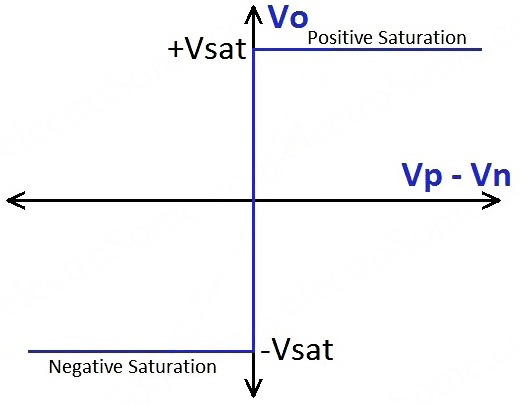
\includegraphics[scale=0.4,valign=t]{idealopampchar.jpg}
		\vphantom{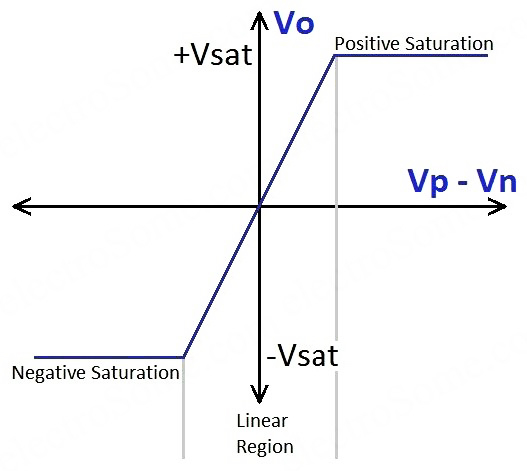
\includegraphics[scale=0.5,valign=t]{opampchar.jpg}}
		
	}
	\subfloat[Non-ideal]{
		\centering
		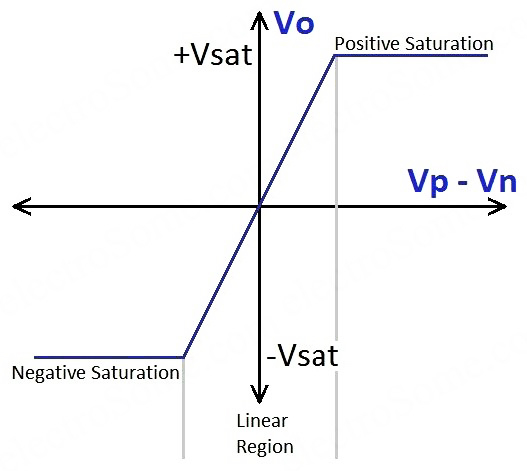
\includegraphics[scale=0.4,valign=t]{opampchar.jpg}
	}
	\caption{Operational amplifier (opamp) characteristics}
	\label{fig:opampchar}
\end{figure}


In an ideal operational amplifier (opamp), it has 2 input channel (inverting ``$-$" and non-inverting ``$+$"). When DC signals flow into these 2 channels, the difference (${V}_{+} - {V}_{-}$) gets amplified with infinite gain (i.e. infinite gradient), only to be limited by supply voltage, reaching saturation voltage ${\text{\pm V}}_{\text{sat}}$. In a non-ideal case, the gain is limited, which means we see a finite gradient.


\begin{figure}[H]
	\centering
	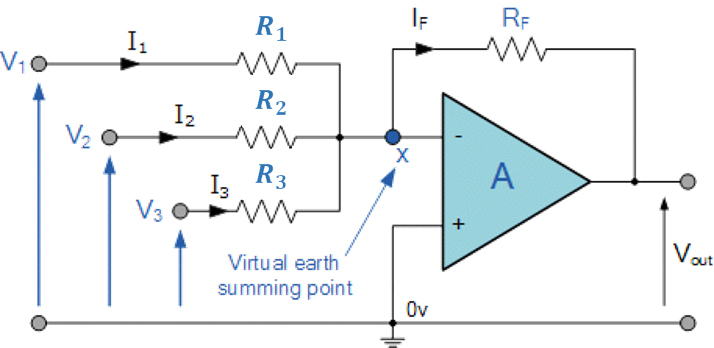
\includegraphics[scale=0.7]{idealsummingopamp.png}
	\caption{Ideal inverting summing opamp}
	\label{fig:noninvertsum}
\end{figure}
In an ideal inverting summing opamp (Figure \ref{fig:noninvertsum}), non-inverting input is grounded. inverting input exhibit a critical virtual ground behaviour. Virtual ground here means, it is not actually grounded, but its voltage is $0V$, and also, no current flows into it. So, based on Kirchoff's Current Law, which states that sum of all current flowing in to a node equals to sum of current flowing out of a node. $I_1$, $I_2$, and $I_3$ flowing into a node marked ``x" in the diagram, since they cannot flow into non-inverting input, all of them flow out as $I_F$ into $R_F$. Since voltage at node x is 0, and a current only flow from low potential to higher potential, we expect $V_{\text{out}}$ to be negative, where the magnitude of $V_{\text{out}}$ equal sum of all current multiplied by $R_F$. Concretely,
$$V_{\text{out}} =-R_F\left( \frac{V_1}{R_1} + \frac{V_2}{R_2} + \frac{V_3}{R_3} \right)$$
Given 3 weights of $w_1$, $w_2$ and $w_3$, we would want: $$\boxed{V_{\text{out}} = w_1V_1+w_2V_2+w_3V_3}$$
So, given $R_F=1$, $w_1$, $w_2$ and $w_3$ correspond to $\frac{1}{R_1}$, $\frac{1}{R_2}$ and $\frac{1}{R_3}$, it infers that: $$w\propto\frac{1}{R}$$
Now, we have:
$$V_{\text{out}}' =-\left( \frac{V_1}{R_1} + \frac{V_2}{R_2} + \frac{V_3}{R_3} \right)$$
To obtain a positive $V_{\text{out}}$, we can go through the same procedure again (attach another opamp to the existing opamp output):
\begin{equation} \label{eq:finalsimplified}
V_{\text{out}} =-R_F'\left( \frac{V_{\text{out}}'}{R_{\text{out}}'} \right)
\end{equation}
When we set $R_F'=R_{\text{out}}'$, we obtain below as needed:
\begin{equation} \label{eq:final}
V_{\text{out}} =-V_{\text{out}}'=\frac{1}{R_1}V_1 + \frac{1}{R_2}V_2 + \frac{1}{R_3}V_3
\end{equation}
Of course, there are many practical issues when we implement the theory above to simulation circuit. This is be covered in Challenges section later on.
\subsection{Simulation Environment}
\begin{figure}[H]
	\centering
	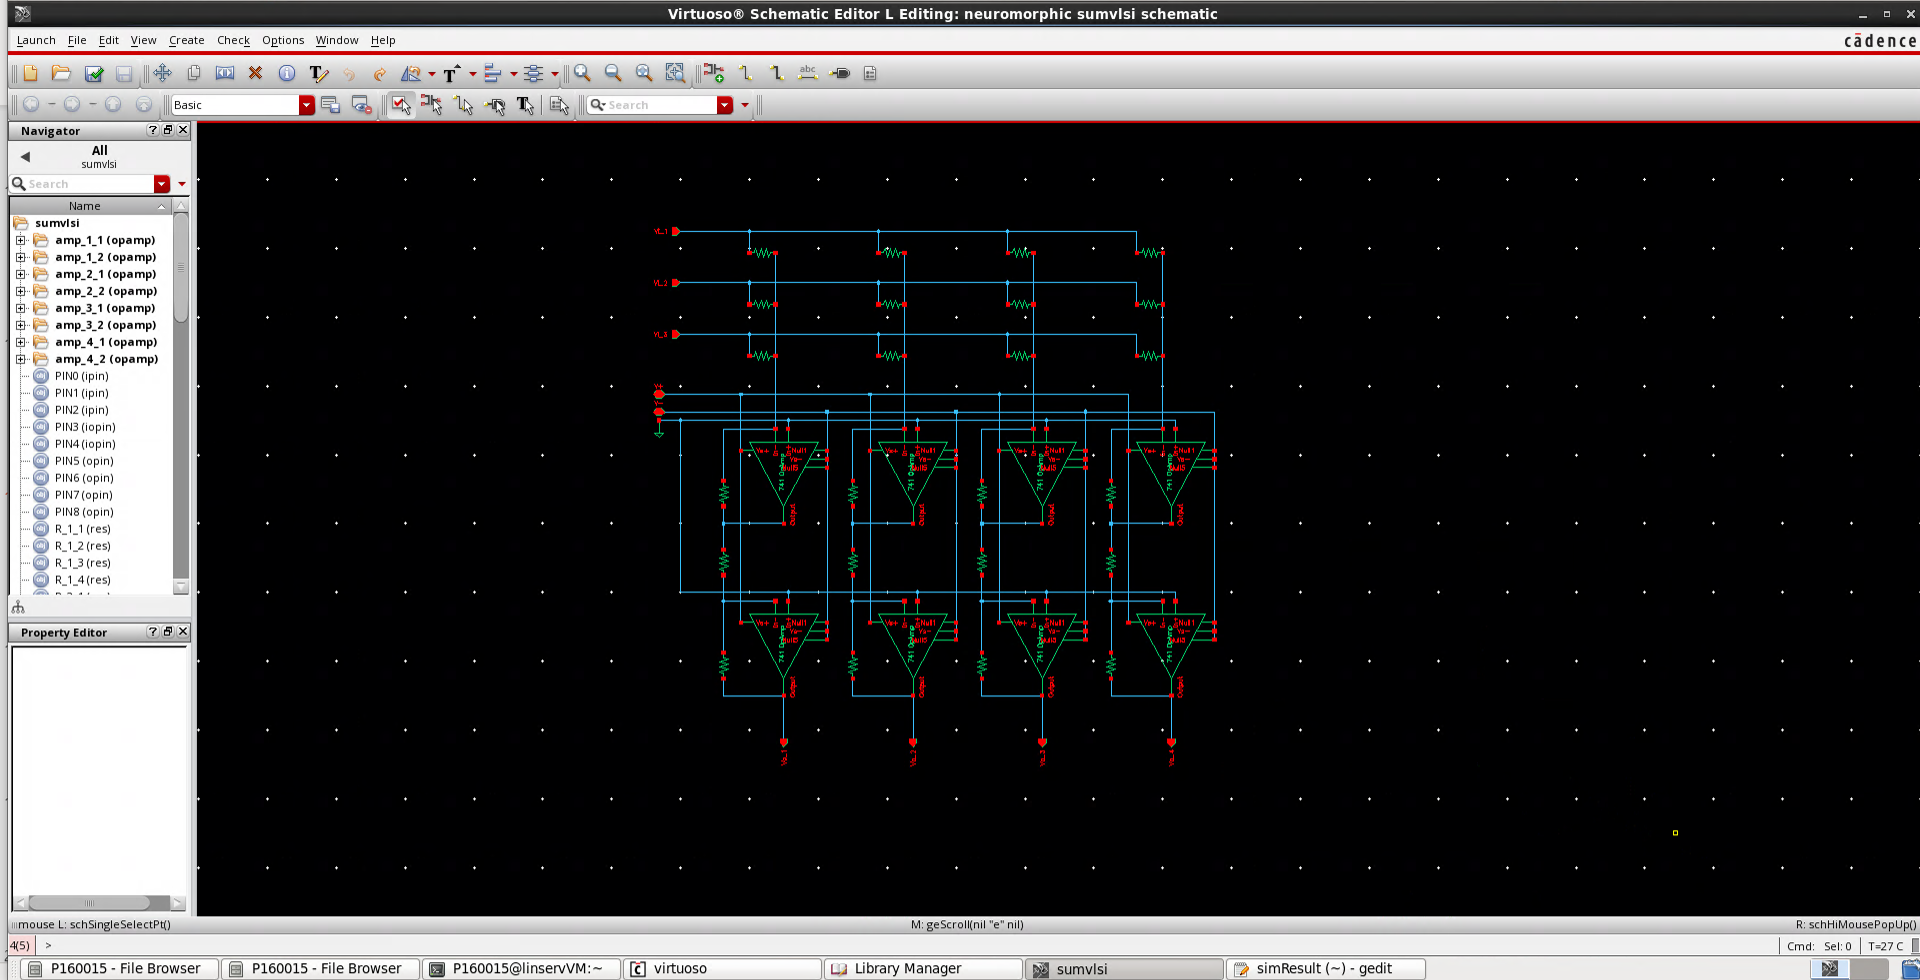
\includegraphics[scale=0.3]{cadence.png}
	\caption{Cadence Design Environment}
	\label{fig:cadence}
\end{figure}
Cadence environment is very powerful for us to build and simulate circuit, even for very large scale simulation. For instance, we can build silicon level layout, fill in the physics details and represent it in a symbolic form. This symbolic form can be used as circuit component in a schematic circuit. Also, we can represent a simple schematic circuit in a symbolic form too, and use it as circuit component in an even larger schematic circuit. The 8 opamps as shown in \ref{fig:cadence} are represented with triangle symbols with input and output pins. Besides, it is entirely possible to simulate a component with just programming its behaviour using scripting language with mathematical and physics description, like spiceText, verilogA, and etc.

Cadence has its own scripting language for automating schematic circuit diagram design, known as Skill Script. Automation functionality extends to component placement by specifying coordinates, rotation, vertical and horizontal flipping, instance id, resistance value, methodical wiring routing and etc. A subset of Skill Script is Ocean Script, meant for automating the testing of the design. For example, in Skill script, we can set the resistance value, input voltage signal to variables (i.e. not hardcoded), so during simulation, we can use Ocean Script to manipulate these variables to automate a sequence of simulations.
\begin{figure}[H]
	\centering
	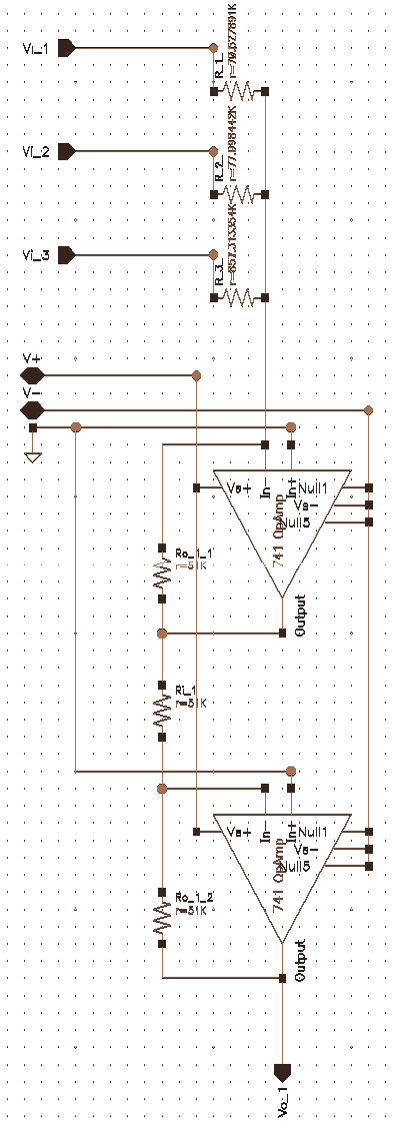
\includegraphics[scale=0.5]{single.png}
	\caption{Single summing neuron implemented in Cadence}
	\label{fig:singleneuron}
\end{figure}
In Figure \ref{fig:singleneuron}, we implemented a single summing neuron with 3 voltage source inputs. The diagram was hand-drawn initially before we moved to programmatic schematic design generation. To ensure minimal errors, all resistance values are hardcoded and the expected neuron output ($V_{\text{out}}$) was calculated manually. Then, Cadence Virtuoso Analog Design Environment (ADE) simulator was used to feed in the voltages (supply voltages inclusive) and measure the output. ADE also allowed us to specify any wiring to measure its voltage and specify the endpoint of any circuit schematic component to measure its current. Current flowing into the specified endpoint is rated positive, whereas the current flowing out is rated negative. Of course, the readout value contains errors, not exactly as calculated. We will cover these errors in our challenges section.